\section{Results and Discussion}
\subsection{Binary--mixture confined between two walls}\label{Piston}
Initially a binary--mixture of two fluids confined between two walls was studied. 
This corresponds to the physical case of a liquid sandwiched between two plates.
The fluid was prepared as described in Section \ref{SystemPrep} at a pressure of $P^{*} = 0.1$ and temperatures of $T^{*} = 0.8$ and $T^{*} = 0.9$.
The confining walls were used as a piston to control the pressure.

\subsubsection{Using the Virial stress}\label{VirialStressPiston}
Once equilibrated, the simulations were run for $40 \times 10^{6}$ timesteps and the number--density and Virial stress--tensor were computed every timestep.
These values were then time-averaged to produce profiles for the number--density and $\sigma_{xx}(z^{*})$ expressed in terms of the scaled coordinate, $z'$, as shown in Figures \ref{PisVirRho} and \ref{PisVirStress}. 

\FloatBarrier
\begin{figure*}[h]
\centering
\includegraphics[scale=0.8]{PisVirRho}
\caption{The number density for the two fluids at $T^{*} = 0.8$ and $T^{*} = 0.9$ is shown. 
The bulk density is uniform, representing a fluid state, and the interface can be seen as the sharp change in the densities of the two fluids.
Near the wall there are oscillations in the density, representing structural layering of the fluid.}
\label{PisVirRho}
\end{figure*}

\begin{figure*}[h]
\centering
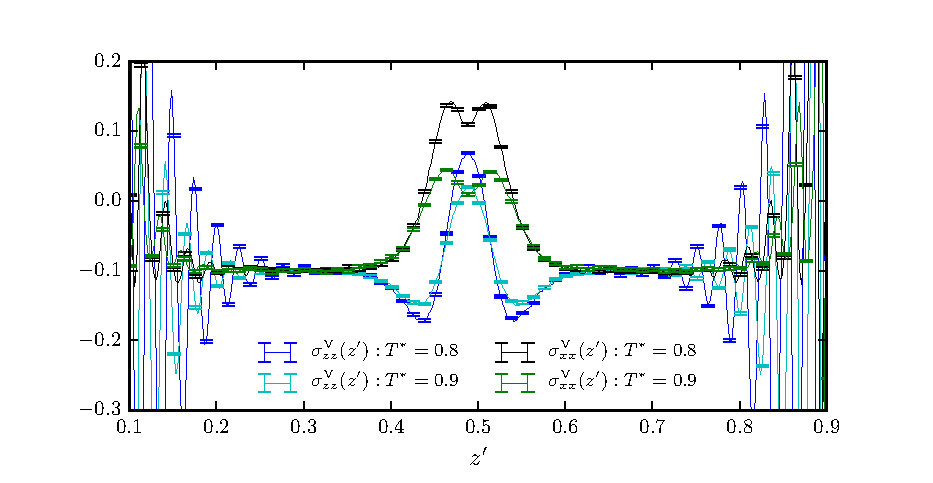
\includegraphics[scale=0.8]{PisVirStress}
\caption{The Virial stress tensor for the total fluid at each temperature shows a bulk value equal to $-P_{ext}$, representing the hydrostatic pressure, and a peak at the interface due to the anisotropy of the interparticle forces in this region.
This peak is related to the interfacial tension and its temperature dependence is the driving force for the Marangoni effect.
Towards the wall there are temperature dependent oscillations which may provide the origin of the thermocapillary force.
PisVirStress caption goes here.}
\label{PisVirStress}
\end{figure*}

Both the density profile and the stress--profile show the expected features of a binary--mixture. 
There is a uniform density in the bulk of the fluid and an interfacial region of finite width where the density of one species falls sharply and the density of the other increases.
Close to the walls, there are large oscillations in the density that are a consequence of structural layering in the fluid close to the solid.
For the stress--profile, the bulk value for the tangential component is equal to $-P_{\mathrm{ext}}$, corresponding to the hydrostatic pressure of the fluid.
At the interface there is a peak in the tangential stress due to the anisotropy of the intermolecular forces in this region, this can be related to the interfacial tension.\cite{Marchand2011}

The time--averaged values for the stress--tensor were then used to estimate the gradient of the stress--tensor with respect to temperature using Equation \ref{FinDiff}, as shown in Figure \ref{PisVirForce}.
This gradient also shows a peak at the interface of the two fluids, providing the origin of the Marangoni force.
Importantly the gradient in the bulk of the fluid (far from both the interface and the walls) is zero within statistical error, ensuring there is no force acting in the bulk fluid.
In addition, there is an oscillating gradient at the surface of the wall which can be interpreted as a thermocapillary force.
Since we are only interested in simulating the Marangoni effect, these thermocapillary forces were ignored.

\begin{figure*}[h]
\centering
\includegraphics[scale=0.8]{PisVirForce}
\caption{The gradient of the Virial stress--tensor with respect to temperature shows a significant negative peak at the interface.
This will generate a force in the opposite direction to a temperature gradient, creating a Marangoni flow.
The oscillations at the liquid--solid boundaries create a thermocapillary force and are ignored.}
\label{PisVirForce}
\end{figure*}
\FloatBarrier

The central $1/3$ of the force profile was then used to create an artifical Marangoni force using a temperature gradient of $\partial T^{*} / \partial x^{*} = 0.001$ and Equation \ref{ForceStressTemp}.
This artfical body force was applied to an identical system prepared at $T^{*} = 0.85$.
A non-equilibrium simulation of this system was run for $40 \times 10^{6}$ and the time--average of the x--component of the fluid velocity, $v^{*}_{x}(z')$, was computed.
The momenta of the walls in the $x$ and $y$ directions were fixed such that they provided a stationary reference point for the fluid.
As a result, the fluid shows non-slip boundary conditions and the walls act to hold the bulk fluid at rest.

\begin{figure*}[h]
\centering
\includegraphics[scale=0.8]{PisVirFlow}
\caption{The fluid velocity generated from a non--equilibrium simulation with an applied artifical Marangoni force calculated from the Virial stress shows a peak at the interface.
The flow direction of this peak is from warm regions to cold.
The greatest velocity magnitude is around 0.16 and this decays linearly to zero at the surface of the piston, corresponding to a Couette flow.}
\label{PisVirFlow}
\end{figure*}
The flow profile calculated for the fluid in this system is shown in Figure \ref{PisVirFlow}. 
There is a sharp negative peak at the interface of the two fluids indicating a Marangoni flow in the opposing direction to the temperature gradient.
Furthermore the flow decays linearly away from the interface, consistent with a Couette flow arising from shear--driven fluid motion.\cite{FluidMech}
There is also a net flow of the fluid, suggesting an overall force acting on the liquid.
The walls in the system act as a momentum sink, providing a friction force on the fluid which allows this steady--state flow to arise under the isolated effect of a temperature--gradient.
\FloatBarrier

\subsubsection{Comparing to the Irving--Kirkwood stress}
Figure \ref{PisVirRho} shows there are significant deviations in the fluid density at the interface and the walls and that the amount of deviation varies with temperature.
Because of the strong dependence of the Virial stress on the local density of the fluid, there is the potential for these changes to interfere with the measurement of the Marangoni force.
To verify the significance of these deviations, the stress--tensor was also calculated using the Irving--Kirkwood formula, since this does not depend on the local fluid density.

\begin{figure*}[h]
\centering
\includegraphics[scale=0.8]{PisIKStress}
\caption{The Irving--Kirkwood stress--tensor shows a similar profile to the Virial stress--tensor (see Figure \ref{PisVirStress}) although the interfacial peak is divided into two and a reduction in the stress occurs directly at the interface.
%This represents the reduction in the momentum flux across the interfacial plane as a result of the weaker interaction between non--equivalent fluid particles.
There are also similar oscillations at the wall due to a thermocapillary force.}
\label{PisIKStress}
\end{figure*}
\FloatBarrier
The fluids were prepared at $P^{*}=0.1$ and $T^{*}=0.8$ and $T^{*}=0.9$ as before.
Since the Irving--Kirkwood stress--tensor takes much longer to compute (see Section \ref{CalcStress}), the equilibrium simulations were only run for $1 \times 10^{6}$ timesteps, resulting in a greater amount of statistical error.
This produced the time--averaged stress--tensor profiles shown in \ref{PisIKStress}.
\FloatBarrier

\begin{figure*}[h]
\centering
\includegraphics[scale=0.8]{PisIKForce}
\caption{The gradient of the Irving--Kirkwood stress--tensor with respect to temperature shows a peak across the interfacial region, representing the origin of the Marangoni force. This occurs with a similar maginitude to the gradient of the Virial stress--tensor although like the stress profile, the Irving--Kirkwood gradient is split into two peaks.
In both gradient profiles, there is no net gradient in the bulk and thus there will be no body force acting in the fluid bulk.}
\label{PisIKForce}
\end{figure*}
The finite difference method was again used to calculate the gradient of this stress--tensor with respect to temperature and this is compared to the Virial result in Figure \ref{PisIKForce}.
Still focussing on only the central $1/3$ of the fluid, there is a good correspondence between the two gradient profiles and the interfacial peak occurs both across the same spatial region and with the same maximum value.
The most signifcant difference occurs directly at the interface, where there is a sharp reduction in the Irving--Kirkwood gradient.
This is probably a result of the reduction in density at the interface affecting the Virial stress--tensor more than the Irving--Kirkwood stress--tensor.
\FloatBarrier

\begin{figure*}[h]
\centering
\includegraphics[scale=0.8]{PisIKFlow}
\caption{The flow profile calculated using the Irvining--Kirkwood Marangoni flow shows a similar profile to that calculated from the Virial force, with a sharp peak at the interface and a linear Couette flow into the bulk.
The peak value is not as large as that from the Virial force as a result of the sharp reduction of the Irving--Kirkwood stress gradient directly at the interface.
The Virial flow is symmetric whilst the Irving--Kirkwood flow is not, this is probably a result of the greater degree of noise in the Irving--Kirkwood gradient due to a short simulation time.}
\label{PisIKFlow}
\end{figure*}
Using a temperature gradient of $\partial T^{*} / \partial x^{*} = 0.001$ to compute the Irving--Kirkwood aritifical body force, a non--equilibrium simulation at $T^{*} = 0.85$ was run for $40 \times 10^{6}$ timesteps.
The flow profile was calculated and compared to the reslult obtained using the Virial force, as shown in Figure \ref{PisIKFlow}.
The profiles show a reasonably good correspondence, especially for the region $z' \leq 0.4$, although they deviate for higher values of $z'$.
In particular the flow from the Irving--Kirkwood force is not as large directly at the interface, as a result of the reduction in the force at this point.
The Irving--Kirkwood velocity profile is also assymetric despite the symmetry of the system.
This assymmetry may be the result of an increase in the noise of the Irving--Kirkwood force relative to the Virial force, which results from the shorter simulation time enforced by the high computational cost of the Irving--Kirkwood analysis.

\subsection{Binary--mixture periodic in 3-dimensions}
Equation \ref{NavierStokes} showed that the existence of a temperature gradient in the system should not be able to generate a net flow in the fluid. 
Levich discusses this further, describing how the interfacial flow must be accompanied by a back-flow in the bulk fluid.\cite{Levich}
In the case of the binary--mixture held between two walls, the stationary walls provide a momentum sink which allows a net flow to exist within the fluid.
To replicate the behaviour described by Levich, a system void of momentum sinks must be studied, for example a binary--mixture of two immiscible fluids with periodic boundary conditions in all dimensions.

This system, shown on the left--hand side of Figure \ref{SetUp}, was prepared as described in Section \ref{SystemPrep} with the parameters given in Section \ref{InteractionModel}.
The distance between consecutive interfaces was $0.5 L_{z^{*}}$.
A Nos\'{e}--Hoover barostat and thermostat were used to control the pressure at $P^{*} = 0.1$ with temperatures of $T^{*}=0.8$ and $T^{*}=0.9$.

\subsubsection{Comparing the Virial and Irving--Kirkwood stress}
There is again an ambiguity over which stress--tensor should be used for computing the Marangoni force.
Initially, the equilibrated symmetric binary--mixture was simulated for $10 \times 10^{6}$ timesteps and the number--density, $\sigma^{\mathrm{V}}$ and $\sigma^{\mathrm{IK}}$ were computed.
As discussed before, the Irving--Kirkwood analysis was highly computationally expensive and this simulation length was the upper feasible limit.
\FloatBarrier

\begin{figure}[h]
\centering
\includegraphics[scale=0.8]{Period10Rho}
\caption{The number--density of the component fluids at $T^{*}=0.8$ and $T^{*}=0.9$ shows a binary--mixture with the interface at around $z'=0.5$.
With the periodic boundary conditions, there are two interfaces per simulation box.
The number density falls at higher temperature and the position of the interface is slightly shifted, this shift must be removed before calculating the stress--gradient.}
\label{Period10Rho}
\end{figure}
After this period, the density profile (plotted in Figure \ref{Period10Rho}) showed a uniform density in the fluid bulk and a sharp interfacial region as expected.
However, the exact position of the interface had shifted during the simulation and was no longer coincedent for the two temperatures.
To calculate the Marangoni force from the stress profile, this shift was manually removed by recentering the interfaces prior to computing the finite difference.
\FloatBarrier

\begin{figure}[h]
\centering
\includegraphics[scale=0.8]{Period10VirStress}
\caption{The tangential component of the Virial stress--tensor shows a bulk value of $-P_{ext}$ and a peak at the interfaces due to the anisotropy of the interparticle fluids at these points.
This peak has a similar form to that seen in the fluid confined between two wall, seen in Figure \ref{PisVirStress}.
}
\label{Period10VirStress}
\end{figure}

\begin{figure}[h]
\centering
\includegraphics[scale=0.8]{Period10IKStress}
\caption{Similarly to Figure \ref{PisIKStress}, the Irving--Kirkwood stress for the binary--mixture periodic in three dimensions matches the Virial stress closely except directly at the interfaces.
The Irving--Kirkwood and Virial stress both show peaks of a similar magnitude and spatial coverage but the peak in the Irving--Kirkwood stress is again split into two peaks.
}
\label{Period10IKStress}
\end{figure}
The recentered Virial and Irving--Kirkwood stress profiles are plotted in Figures \ref{Period10VirStress} and \ref{Period10IKStress} respectively.
As with the fluid confined between two walls, the bulk stress--tensor components are equal to $-P_{\mathrm{ext}}$, correpsonding to the hydrostatic fluid pressure.
There is a similar peak in both the Virial and Irving--Kirkwood stress at the interface.
The peaks also have the same maximum value for both stress--tensors, although the Irving--Kirkwood stress shows a stronger minimum directly at the interface.
Similarly to Figure \ref{PisIKStress}, this is probably the result of a reduced density in the interfacial region.

\FloatBarrier
Using these stress profiles, the gradient of the stress with respect to temperature was calculated through the finite difference approach.
For there to be no net force acting on the fluid, the gradient profile was adjusted by subtracting the average value from each point to ensure the intergral over all space was zero, as shown in Figure \ref{Period10Force}.
This replicated the effect of a momentum sink in the infinite periodic fluid, for example a distant boudning wall.

\begin{figure}[h]
\centering
\includegraphics[scale=0.8]{Period10Force}
\caption{The gradient of the stress--tensor with respect to temperature calculated using equilibrium simulations of $10 \times 10^{6}$ timesteps shows the expected peak at the interfaces. 
This profile was adjusted to give no net gradient by subtracting the average gradient.
There appears to be a good correspondence between the Irving--Kirkwood and Virial stress--gradients, however such a short simulation timescale gives a large amount of noise in this gradient profile.
Consequently, the gradient profiles are not sufficiently precise to use for calculating an artificial body force and applying this to a non--equilibrium simulation.
}
\label{Period10Force}
\end{figure}
The resulting gradient profile shows a similar peak at the interface to Figure \ref{PisIKForce}. 
The maximum values are similar, suggesting that fixing the total force to zero correctly adjusts the data to give a physically meaningful Marangoni force.
Again there is a reasonably good correspondence between the gradient calculated from the Irving--Kirkwood and Virial stress--tensors, and the magnitude of the Irving--Kirkwood peak is reduced directly at the interface.
There is also a bulk gradient acting in the opposite direction to the interfacial peak, generating the predicted back force which balances the Marangoni force.
However, the profile as a whole shows too much noise for the fine--structure to be determined and is not of a sufficient quality to be used in calculating an artificial body--force.

\subsubsection{Reducing the noise in the force--profile}
To generate a gradient profile with a sufficiently low level of nosie requires either a larger system size or a longer simulation time.
Both of these increase the computational cost of calculating the Irving--Kirkwood stress--tensor beyond a practical level and the Virial stress--tensor must be used.
Considering how similar the Virial and Irving--Kirkwood gradient profiles appear in Figure \ref{PisIKForce}, using the Virial stress--tensor does not create too much deviation from the more suitable Irving--Kirkwood stress--tensor whilst enabling a much longer simulation time.
\FloatBarrier

\begin{figure}[h]
\centering
\includegraphics[scale=0.8]{Period30VirStress}
\caption{Running the equilibrium simulation over $30 \times 10^{6}$ timesteps produced a much more precise Virial stress profile with a significant reduction in noise relative to Figure \ref{Period10VirStress}.
The noise in the bulk stress lies within statistical error and thus is consistent with the hydrostatic pressure.
This simulation time is too long for the Irving--Kirkwood method to be feasible.
}
\label{Period30VirStress}
\end{figure}

The reduced noise stress--profile was generated by running the equilibrium systems for $30 \times 10^{6}$ timesteps.
Recentering the interfaces generated the Virial stress profile shown in Figure \ref{Period30VirStress}.
For both temperatures, the profiles show much less noise compared to Figure \ref{Period10VirStress}, especially in the bulk region, and the interfacial peaks are more symmetric.
\FloatBarrier

\begin{figure}[h]
\centering
\includegraphics[scale=0.8]{Period30VirForce}
\caption{The Virial stress gradient calculated using equilibrium simulations of $30 \times 10^{6}$ timesteps showed significantly less noise than the equilibrium simulations of $10 \times 10^{6}$ timesteps.
Having subtracted the average value to give no gradient overall, the plot confirms there is a sharp and symmetrical interfacial peak with an opposing gradient in the fluid bulk.
}
\label{Period30VirForce}
\end{figure}
Using these stress profiles, the gradient of the stress--tensor with respect to temperature was again computed using the finite difference and the average value subtracted to give the profile shown in Figure \ref{Period30VirForce}.
There is a dramatic reduction in the noise of this gradient profile compared to Figure \ref{Period10Force} and there is definitely a sharp peak at the interface with an opposing gradient in the bulk regions.
\FloatBarrier

Using the gradients given in Figure \ref{Period30VirForce} and a temperature gradient of $\partial T^{*} / \partial x^{*} = 0.001$, an artifical body force was computed.
The body force was recentered to ensure that the peak corresponding to the Marangoni force aligned with the interfacial region, and was applied in a non--equilibrium simulation at $T^{*} = 0.85$.
This simulation was run for $40 \times 10^{6}$ and $v^{*}_x(z')$ was computed to yield the flow profile plotted in Figure \ref{Period30VirFlow}.

\begin{figure}[h]
\centering
\includegraphics[scale=0.8]{Period30VirFlow}
\caption{The flow profile calculated from a non--equilibrium simulation using the stress gradient shown in Figure \ref{Period30VirForce} and a temperature gradient of $\partial T^{*} / \partial x^{*} = 0.001$ has a large amount of noise and is not very conclusive.
There is a net flow velocity despite the average gradient being set to zero, it is unlikely this could be improved upon without artificially fixing the centre--of--mass.
Despite this, the fluid velocity relative to this centre--of--mass motion suggests a negative peak at the interfaces with some back flow in the bulk regions, satisfying Levich's requirement of a stationary net flow.\cite{Levich}
 }
\label{Period30VirFlow}
\end{figure}

Despite the simulation being run for a long timescale, this flow profile still retains a lot of statistical noise.
It would be difficult practically to reduce this noise further.
Moreover the average velocity (indicated the hashed line) is non--zero, implying that there is centre--of--mass motion during the simulation.
This motion is occuring even though the gradient--profile has been recentered to give no net force overall.
It is likely that in the absence of a momentum sink for a system like this, it would be very difficult to completely remove this net flow without artificially fixing the centre--of--mass throughout the simulation.

Despite this, the relative motion across the fluid can still be considered and there does appear to be a velocity peak at the interface (with $v < v_{\mathrm{COM}}$) corresponding to a Marangoni flow, and a back flow in the bulk fluid (with $v > v_{\mathrm{COM}}$) as predicted.
This result is, however, somewhat ambiguous and there was insufficient project time to improve the non--equilibrium simulation further.

\subsection{The effect of surfactants}
Surfactant molecules decrease the surface free energy of interfaces, as they have a favourable interaction with both fluids and bridge the interfacial plane.
This reduction in surface--tension should also cause a decrease in the Marangoni effect, as observed experimentally.\cite{KimSubramanianA,KimSubramanianB,BartonSubramanian,ChenStebe}

To model this, the non--ionic surfactant molecules described in Section \ref{ModellingSurfactants} were added to the binary--mixture confined between two walls.
This system was chosen since the results of Section \ref{Piston} showed it allowed a steady--state flow to be generated and modelled effectively.

The surfactant molecules were added to a single plane between the two fluids in the initial lattice (before equilibration).
A certain fraction of these molecules were then removed to vary the surfactant concentration, quantified as a fraction of the total number of fluid particles present,
\begin{equation}
\mathrm{Surfactant\ Fraction} \equiv \frac{N_{\mathrm{surfactant}}}{N_{\mathrm{surfactant}}+N_{\mathrm{fluid}}}
\end{equation}
This allowed the surfactant fraction to be varied between $0$ and $0.00323$.

Taking surfactant fractions of $0.000$, $0.0031$, $0.0098$, $0.0194$, $0.0264$, $0.0298$ and $0.0323$, the fluid was then prepared as described in Section \ref{SystemPrep} with a pressure of $P^{*}=0.1$ and temperatures of $T^{*}=0.8$ and $T^{*}=0.9$.
A piston barostat and Nos\'{e}--Hoover thermostat were used and each system was run at equilibrium for $30 \times 10^{6}$ timesteps of length $0.001\ \tau$.

\begin{figure}[h]
\centering
\includegraphics[scale=0.8]{SurfRho}
\caption{The number density for the binary--mixture with nonionic surfactant molecules, at  $T^{*}=0.8$ and with a surfactant fraction of $0.0194$, is plotted.
There is a uniform density in the bulk, showing a fluid like state, and a sharp interface where the densities of Fluid A and Fluid B change rapidly.
The surfactant particles are localised at the interface with a low solubility.
They also show the correct orientation, with `Head' particles interacting most strongly with Fluid A and `Tail' particles with Fluid B.
}
\label{SurfRho}
\end{figure}

The resulting number density of each species shows a uniform bulk density, a sharp interface and peaks for the Head and Tail groups located at the interface, as shown for $T^{*}=0.8$ and a surfactant fraction of $0.0194$ in Figure \ref{SurfRho}.
At the interface, the surfactant molecules were correctly oriented with respect to Fluid A and Fluid B.
\FloatBarrier

\begin{figure}[h]
\centering
\includegraphics[scale=0.8]{SurfForce}
\caption{The gradient of the Virial stress--tensor for the surfactant systems still shows a strong interfacial peak for a low surfactant fraction.
As the amount of surfactant is increased, the strength of this peak decreases to zero with a resulting reduction in the Marangoni force.
}
\label{SurfForce}
\end{figure}

The Virial stress--tensor was computed during the equilibrium simulations and used to compute the gradient of the stress with respect to temperature for each surfactant fraction.
These results are plotted in Figure \ref{SurfForce} show a pronounced reduction in the magnitude of the interfacial peak as the surfactant fraction increases.
This corresponds to the expected reduction in the Marangoni force at the interface.
Two smaller peaks on either side of the central peak also develop for higher surfactant fractions.
These potentially correspond to an opposing force driven by a gradient in the surfactant concentration which becomes significant at high surfactant fractions.
Further investigation would be needed to confirm the origin of this peak.
\FloatBarrier

\begin{figure}[h]
\centering
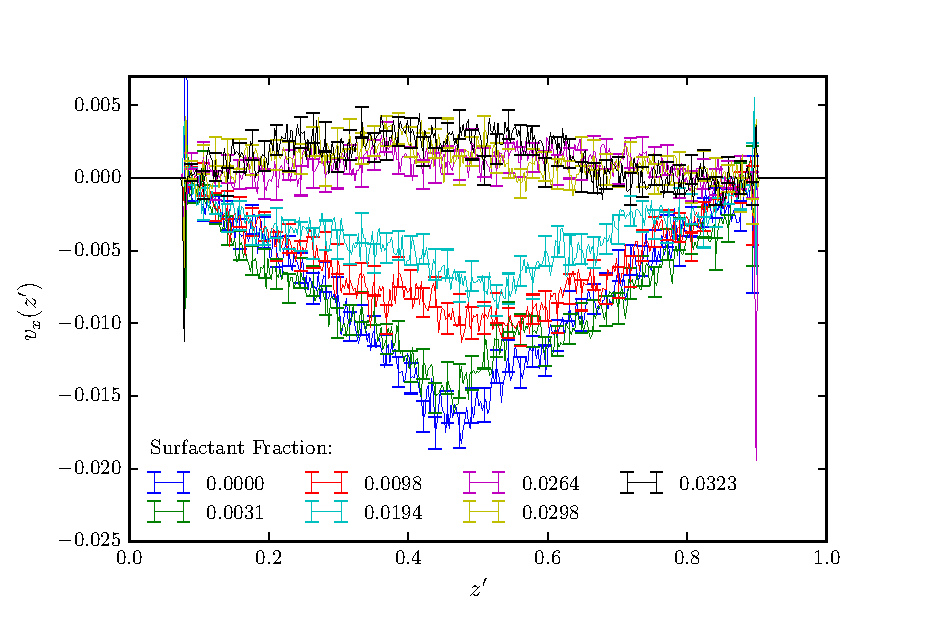
\includegraphics[scale=0.8]{SurfFlow}
\caption{For a low surfactant fraction, the flow profile closely resembles that of the non--surfactant system with an interfacial peak and a linear decay into the bulk.
As the amount of surfactant increases there is a reduction in the magnitude of this peak until the Marangoni flow is essentially removed.
}
\label{SurfFlow}
\end{figure}
Using a temperature gradient of $\partial T^{*} / \partial x^{*} = 0.001$, the central $1/3$ of the stress--gradients in Figure \ref{SurfForce} where used to caculate an artificial body force which was applied in a non--equilibrium simulation at $T^{*}=0.85$.
These simulations were run for $30 \times 10^{6}$ timesteps over which $v_{X}(z')$ was computed and plotted in Figure \ref{SurfFlow}.
There is a clear decrease in the interfacial velocity as the surfactant fraction is increased.

The sharpness of the Marangoni flow peak is also decreased and no longer fits the Couette model as conclusively as when no surfactant molecules are present.
This may be because the surfactant molecules decrease the viscosity at the interface, giving non-uniformity across the fluid. 
To confirm this, the viscosity could be measured using the Green--Kubo relation,
\begin{equation}
\eta = \frac{1}{V k_{\mathrm{B}} T} \int_{0}^{\infty} \left< \sigma_{xy} \left( \tau \right) \sigma_{xy}(0) \right> \mathrm{d} \tau.
\end{equation}

\FloatBarrier
\begin{figure}[h]
\centering
\includegraphics[scale=0.8]{InterVel}
\caption{As the surfactant fraction in the system increases, the magnitude of the interfacial velocity decreases.
Above a fraction of $0.025$, this velocity is essentially zero, although there is small velocity in the opposite direction to the Marangoni flow.
This backwards velocity may be the result of a gradient in the amount of surfactant at the interface, which could occur as the surfactant molecules will be more soluble at higher temperatures so will have a smaller interfacial excess.
Such an effect may only be significant for high surfactant concentrations.
}
\label{InterVel}
\end{figure}
The interfacial velocity can be taken as the velocity of the profile peaks in Figure \ref{SurfFlow}.
Comparing these values against the surfactant fraction shows a clear reduction in the magnitude of this peak value as the surfactant fraction increases, as shown in Figure \ref{InterVel}.
Above a fraction of $0.025$ it appears the Marangoni effect has been removed completely, matching the experimental observations well.
\FloatBarrier
